\chapter{Results}
\label{ch:res}

In this chapter we explain how we use the forward model to generate data and how we set up a Bayesian framework to then give distribution of solutions.
Here we make it explicit and proivde all information to be able to replciate our results.
In this work we simulate datawith an ozone profile from \cite{}.
We follow the U.S. standard atmosphere, 1976 \cite{} to relate pressure and temperature and hieght and the HITRANonline \cite{} database to calculate the measured signal.\expandafter\string\the\font 

\section{Simulate Data}
\begin{figure}[ht!]
	\centering
	\input{LIMB.pdf_tex}
	\label{fig:LIMB}
	\caption{Schematic of measurement and analysis geometry, not to scale.
		The stationary satellite, at a constant height $h_\text{sat}$ above  Earth, takes $m$ measurements.
		The red dashed lines show the line-of-sight from the satellite for each measurement, defining the line $\Gamma_j$ from the satellite with limb height $\ell_j$, $j=1,2,\dots,m$ (not shown).
		Between $h_0 = 10$km and $h_{n} = 38$km, the stratosphere is discretised into $n$ layers as illustrated by the solid green lines.}
\end{figure}
We put the satellite at a constant observe height of $h_{obs} =$ and take $m = $ along the line of sight $\Gamma_j$ in between $h_0= $ and $h_n = $ as requested by Annika et. al. since the pointing accuracy is .
we assume no signal above and below and that the we have a constant LTE atmosphere in each layer.
As in section \ref{sec:formodel} the atmosphere is discretised into $n = $ layers
Where we take the same discretization as given by an ozone profile taken from NASA's (Microwave limb sounder) MLS \cite{}.



\subsection{Ozone}
\begin{figure}[ht!]
	\centering
	%\scalebox{1}{\input{TrueO3.pdf_tex}}
	\caption{We take the ozone profile from \cite{}, relate pressure and height and discretise according to the source.
		This will serve as our true Ozone profile.}
	\label{fig:nter-label}
\end{figure}
From \cite{} we choose a relatively smooth ozone profile, where each ozone volume mixing ratio corresponds to a distinct pressure values.
Up until $86$km we can relate pressure $p$ and geometric height $h$ through the hydrostatic equation
\begin{align}
	\text{d} \ln p= \frac{\text{d}p}{p} = \frac{- g M}{R^* T} \text{d} h \, ,
\end{align}
with the universal gas consant $R^* \approx 8.314  \, \text{N m} / \text{mol} / \text{K}$. The moledus numebr ... is $M = M_0 \approx 28.97 \, \text{kg}/\text{mol}$ for altiudes below 79km \cite{}.
At altitude $h$ the gravitational constant
\begin{align}
	g = g_0 \Bigg( \frac{r_0}{r_0 + h} \Bigg) \, ,
\end{align}
with $r_0 \approx 6356 \, \text{km}$ (also known as the polar radius of the earth) and $g_0 \approx 9.81 \text{m}/\text{s}^2$ and \cite{}.
\subsection{Pressure}
We parametrize the pressure by fitting one exponential to the pressure values $p$ related to the height $h$ by Eq. \ref{}.
\begin{figure}[ht!]
	\centering
	%\scalebox{1}{\input{TruePress.pdf_tex}}
	\caption{In green the true pressure profile, where we fit two exponential to it.
		Above $h_{p,0}$ the gradient of the epxonetinal is $a_{p,1}$ and below $a_{p,0}$.
		We have a $p_0$ wehere those two expontentials meet}
	\label{fig:nter-label}
\end{figure}
The pressure function,
\begin{align}
	p(h) =
		\exp{ \{ -b \,  (h - h_{0} ) \} } \,  p_0 \, ,
\end{align}
is depending on three different parameters, the gradient $a_{p,1}$ and the tuple $(p_0,h_{p,0})$.


\subsection{Temperature}

\begin{figure}[ht!]
	\centering
	%\scalebox{1}{\input{TrueTemp.pdf_tex}}
	\caption{True temperature profile, in the altitude of interest.
		The gradients $a_0,a_1,a_2,a_3,a_4$ and the corresponding height $h_0,h_1,h_2,h_3,h_4,h_5$ as well as the temperature $T_0$ at $h = 0$ are taken from the us standard atmosphere and parametrize the temperature profile.}
	\label{fig:nter-label}
\end{figure}
We can formulate a temperature function from \cite{atmosphere1976us}
\begin{align}
	T(h) = \begin{cases*}
		T_0 & \text{$h = 0$}\\
		T_0 + a_0 h, & \text{$0 \leq h < h_{0}$}\\
		T_0 + a_0 h_0, & \text{$h_{0} \leq  h < h_{1}$}\\
		T_0 + a_0 h_0 + a_1 (h -h_1) , & \text{$h_{1} \leq h < h_{2}$}\\
		T_0 + a_0 h_0 + a_1 (h_2 - h_1) + a_2 (h - h_2), & \text{$h_{2} \leq h < h_{3}$}\\
		T_0 + a_0 h_0 + a_1 (h_2 - h_1) + a_2 (h_3 - h_2), & \text{$h_{3} \leq h < h_{4}$}\\
		T_0 + a_0 h_0 + a_1 (h_2 - h_1) + a_2 (h_3 - h_2) + a_3 (h -h_4), & \text{$h_{4} \leq h < h_{5}$}\\
		T_0 + a_0 h_0 + a_1 (h_2 - h_1) + a_2 (h_3 - h_2) + a_3 (h_4 - h_4) + a_4 (h -h_5), & \text{$h_{5} \leq h < 84.852\text{km}$}
	\end{cases*} 
\end{align}
depending on 12 parameters with values provided by \cite{}, also see table \ref{}.
We set this as our true temperature profile and refer to \cite{} for temperature values above $79 \,\text{km}$.


\subsection{Source}
We calculate the source function $B(\nu, T)$ and the absorption constant $ k(\nu, T)$ as follows.

For one species at one specific wave-number the weighted absorption constant becomes
\begin{align}
	\overline{k(\nu, T, r)}    = \sum_{m=1}^{molec} k_m(\nu, T) x_m(r) =  k(\nu, T) x(r) \, ,
\end{align}
with the volume mixing ratio of ozone $x(r)$ at location $r$. 
The absorption constant
\begin{align}
	k(\nu, T) = L(\nu, T_{\text{ref}}) \frac{Q(T_{\text{ref}})}{Q(T)} \frac{ \exp{\{ - c_2 E^{\prime \prime} / T\}} }{\exp{\{ - c_2 E^{\prime \prime} / T_{\text{ref}} \}}} \frac{ 1- \exp{\{ - c_2 \nu  / T \}} }{1 - \exp{\{ - c_2 \nu / T_{\text{ref}} \}}}
\end{align}
is depend on the line intensity $L(\nu, T_{\text{ref}})$ at reference temperature $T_{\text{ref}} =296K $, the lower-state energy of the transition $ E^{\prime \prime} $, the second radiation constant $c2=1.4387769\text{cmK}$ all provided by \cite{}.
Since we only consider one transition namely the lower-state one the partition function becomes
\begin{align}
	Q(T )= g^{\prime \prime} \exp{\{ - \frac{ c_2 E^{\prime \prime} }{T}\}} \, ,
\end{align}
with the the statistical weight $ g^{\prime \prime}$ (also called the degeneracy factor), see \ref{}.
M. Šimečková, D. Jacquemart, L. S. Rothman, R. R. Gamache, and A. Goldman, "Einstein A-coefficients and statistical weights for molecular absorption transitions in the HITRAN database", J. Quant. Spectrosc. Radiat. Transfer 98, 130-155 (2006)

Under the assumption of local thermodynamic (LTE) equilibrium t source function is given by the black body radiation
\begin{align}
	B(\nu,T)   = \frac{2 h c^2 \nu^3}{\exp{\{\frac{hc\nu}{k_B T}\}}-1}\, ,
\end{align}
with Planck's constant $h$, velocity of light $c$ and Boltzmann's constant $k_B$ \cite{}.

Then we can calculate measurement with the RTE in Eq. \ref{eq:RTE} using the trapezoidal rule.



\section{Bayesian Model and prior analysis}
In this section we present the explicit Bayesian we will use to recover pressure temperature and ozone values.

\subsection{DAG}
Again we draw a DAG and specify prior disribtoin over those

\begin{figure}[thb!]
	\centering
	\begin{tikzpicture}
		\node[roundnode2] at (-4.5,6.5) (Q)     {$\bm{Q}$};
		\node[roundnode2] at (-3,5) (x)     {$\bm{x}$};
		\node[align=center] at (-1,4) (A)    {$\bm{A}(\bm{x},\bm{p},\bm{T})$};
		\node[roundnode2] at (-1,2.5) (u)    {$\bm{u}$};
		\node[rectnode] at (-1,1) (y)    {$\bm{y}$};
		\node[roundnode2] at (-5.25,4.5) (S)    {$\bm{\Sigma}$};
		\node[roundnode2] at (-6.5,6.25) (s)    {$\gamma$};
		\node[roundnode2] at (-5.5,8) (d)    {$\delta$};
		\node[roundnode2] at (3,6.5) (t)     {$\bm{T}$};
		\node[roundnode2] at (-1,6.5) (p)     {$\bm{p}$};
		\node[roundnode2] at (1,5) (pt)     {$\bm{p}/\bm{T}$};
		\node[roundnode2] at (0,8) (b1)    {$b$};
		%\node[roundnode2] at (1,8) (b2)    {$b_2$};
		\node[roundnode2] at (-2,8) (h1)    {$h_0$};
		\node[roundnode2] at (-1,8) (p0)    {$p_0$};
		\node[roundnode2] at (2.25,8) (ht)    {$\bm{h_T}$};
		\node[roundnode2] at (3.25,8) (ct)    {$\bm{c_T}$};
		\node[roundnode2] at (4.25,8) (at)    {$\bm{a_T}$};
		
		%Lines
		\draw[->, mydotted, very thick] (S.south east) -- (y.west);
		\draw[->, very thick] (s.south) -- (S.north west);
		\draw[->, very thick] (u.south) -- (y.north);
		\draw[->, mydotted, very thick] (A.south) -- (u.north);
		\draw[->, mydotted,  very thick] (x.south east) -- (A.west);
		\draw[->, very thick] (p.south east) -- (pt.north west);
		\draw[->, very thick] (t.south west) -- (pt.north east);
		\draw[->,  mydotted, very thick] (pt.south west) -- (A.east);
		\draw[->, very thick] (h1.south) -- (p.north west);
		\draw[->, very thick] (p0.south) -- (p.north);
		\draw[->, very thick] (b1.south) -- (p.north east); 
		%\draw[->, very thick] (b2.south) -- (p.east); 
		
		\draw[->, very thick] (d.south) -- (Q.north west); 
		
		\draw[->, very thick] (Q.south east) -- (x.north west); 
		\draw[->, very thick] (ht.south) -- (t.north west);
		\draw[->, very thick] (ct.south) -- (t.north);
		\draw[->, very thick] (at.south) -- (t.north east);
		%\node[align=center] at (0.25,3.95) (f3) {$\approx \bm{M A}_L$};
	\end{tikzpicture} 
\caption[]{Here $\bm{h_T}$, $\bm{c_T}$,$\bm{a_T}$ are the cuntino parameters}
\end{figure}

\subsection{Prior Modelling}
\begin{table}
	\centering
	\begin{tabular}{ |c||c|c|c|c|   }
		\hline
		& &\multicolumn{2}{|c|}{TT bounds}&\\
		\hline
		model parameters& priors&\makecell{lower}& \makecell{upper\\
		}&Context\\
		\hline
		$\gamma$ & $\mathcal{T}(1,10^{-10})$ &0 &1& $\bm{y}$\\ \hhline{|=||=|=|=|=|}
		$\delta$ &$\mathcal{T}(1,10^{-10})$ & 0&1& $\bm{x}$\\ \hline
		$\bm{x}$ &$\mathcal{N}(0,\delta \bm{L})$ & -&-& $\bm{x}$\\ \hhline{|=||=|=|=|=|}
		%$\gamma$ & $\mathcal{N}(2.58e-9,2.58e-11)$ &2.45e-9&2.7e-9 &$\bm{x}$\\
		%$\delta_0$ &  $\mathcal{N}(0.8e-4,0.75e-5)$& 4e-5 & 1.1e-4&$\bm{x}$\\
		%$a_0$ &  $\mathcal{T}(3,1e6)$& 1e-15&1e-5&$\bm{x}$\\ \hline
		%$h_0$ &  $\mathcal{N}(31.35,1)$&27 &35&$\bm{x}$\\ \hline
		$h_0$ &  $\mathcal{N}(34.3,0.5)$& 32.8&35.64&$\bm{p/T}$\\ \hline
		$p_0$ &  $\mathcal{N}(6.5,0.1)$&6.17 &6.73&$\bm{p/T}$\\ \hline
		$b$ &  $\mathcal{N}(0.15,0.0051)$& 0.138  &0.167&$\bm{p/T}$\\ \hline
		%$b_2$ & $\mathcal{N}(0.13,0.067)$& 0&0.32&$\bm{p/T}$\\ \hline
		$h_{T,0}$ &  $\mathcal{N}(11,0.5)$&9.6 &12.4&$\bm{p/T}$\\ \hline
		$h_{T,1}$ &  $\mathcal{N}(20,3)$&11.6 &28.4&$\bm{p/T}$\\ \hline
		$h_{T,2}$ &  $\mathcal{N}(32,1)$&29.2 &34.8&$\bm{p/T}$\\ \hline
		$h_{T,3}$ &  $\mathcal{N}(47,2)$&41.4 &52.6&$\bm{p/T}$\\ \hline
		$h_{T,4}$ &  $\mathcal{N}(51,2)$&45.4 &56.6&$\bm{p/T}$\\ \hline
		$h_{T,5}$ &  $\mathcal{N}(71,2)$&65.4 &76.6&$\bm{p/T}$\\ \hline
		$a_{T,1}$ &  $\mathcal{N}(-6.5,0.01)$&-6.528 &-6.472&$\bm{p/T}$\\ \hline
		$a_{T,2}$ &  $\mathcal{N}(1,0.01)$&0.972 &1.028&$\bm{p/T}$\\ \hline
		$a_{T,3}$ &  $\mathcal{N}(2.8,0.1)$&2.52 &3.078&$\bm{p/T}$\\ \hline
		$a_{T,4}$ &  $\mathcal{N}(-2.8,0.01)$&-2.828 &-2.772&$\bm{p/T}$\\ \hline
		$a_{T,5}$ & $\mathcal{N}(-2,0.01)$ &-2.028 &-1.972&$\bm{p/T}$\\ \hline
		$t_{0}$ &  $\mathcal{N}(288,2)$& 282.54 &293.75&$\bm{p/T}$\\
		\hline
	\end{tabular}
	\caption{Gaussian $\mathcal{N}(\mu,\sigma)$ and gamma distribution $\mathcal{T}(\alpha = \text{scale}, \beta = \text{rate})$
		Bounds for t and p 2.8 times the variance around the mean
		round pressure approx and  test if would work with previous gamma prior or fix gamma prior with set values}
	\label{tab:1}
\end{table}

\begin{itemize}
	\item prior of ozone (picture), with samples drawn from gamma distr
	\item prior of pressure and temperature
\end{itemize}
In practise we sperate OPzone and conditoin on tempreature and pressure  or vice versa. 
\subsubsection{Ozone}
graph lacoiacn 
wigthing in between
similiar to a ciuop;led osscialtors
what heught is change of weights
\begin{align}
	\bm{Q}= \delta \bm{L} =
	\delta
	\begin{bmatrix}
		2 & -1 & & &  \\
		-1 & 2 & -1 & &   \\
		& \ddots & \ddots & \ddots &\\ 
		&   & -1 & 6 & -5 \\
		& & & \ddots & \ddots & \ddots  \\ 
		& & & &  -5 & 10 & -5 \\
		& & & & & -5 & 10 
	\end{bmatrix}  
\end{align}

\subsubsection{pressure over temperature}


\begin{itemize}
	\item show that pressure is dominant
	\item appendix
\end{itemize}





\subsection{Posterior distributions}
\begin{itemize}
	\item explain where we use MTC and that T/p is spereate
	\item marginal posterior, noise and covarince and perciosn matrix
	\item picture of f and g
	\item taylor expansion
	\item maybe make  metroplis explixit
\end{itemize}
conditioned on a ozone profile
\subsubsection{pressure over temperature}

conditioned on a temperauter opver pressure profile
\subsubsection{Ozone -- marginal posterior}

\subsubsection{Ozone -- conditional posterior}


\section{Affine Map}
\begin{itemize}
	\item explicit, why we need ozone profiles, because it is faster and temperature and pressure are more well defined within the atmosphere
\end{itemize}
We do MTC with linear forward map no updadeted
In this specific case we find the affine map
\begin{align}
	\bm{M} = \begin{bmatrix}
		\text{---} & \bm{M}_0 &   \text{---}  \\
		&  \vdots  & \\
		\text{---}& \bm{M}_j &  \text{---} \\
		&  \vdots  & \\
		\text{---} & \bm{M}_m &   \text{---}
	\end{bmatrix} \, \in \mathbb{R}^{m \times m} ,
\end{align}
with rows $\bm{M}_j$ using a linear solver for
\begin{align}
	W \bm{M}_j^\top \, = V_{j} \, .
\end{align}
Here $V_j$ denotes the $j$th row of  
\begin{align}
	V = \begin{bmatrix}
		\vert&   &  \vert & & \vert \\
		\bm{A}_{NL} (\bm{x}^{(1)} ) &  \cdots& \bm{A}_{NL} (\bm{x}^{(j)} )&  \cdots & \bm{A}_{NL} (\bm{x}^{(m)})  \\
		\vert&   &  \vert & & \vert 
	\end{bmatrix}
\end{align}
and
\begin{align}
	W = \begin{bmatrix}
		\vert&   &  \vert & & \vert \\
		\bm{A}_{L} \bm{x}^{(1)} &  \cdots& \bm{A}_{L} \bm{x}^{(j)} &  \cdots & \bm{A}_{L} \bm{x}^{(m)} \\
		\vert&   &  \vert & & \vert 
	\end{bmatrix}
\end{align}
is a $\mathbb{R}^{m \times m} $ matrix as well as $\bm{A}_{NL}$.
Then the non-linear forward model can be approximated so that
\begin{align}
	\bm{A}_{NL}(\bm{x}) \approx \bm{M A}_L \bm{x}\, .
\end{align}

\subsection{First MTC}
\begin{itemize}
	\item make table with set up for TT and sampling 
	\item normalize in evrey step
\end{itemize}
\begin{figure}[thb!]
	\centering
	\begin{tikzpicture}
	\node[roundnode2] at (-4.5,6.5) (Q)     {$\bm{Q}$};
	\node[roundnode2] at (-3,5) (x)     {$\bm{x}$};
	\node[align=center] at (-1.55,4) (A)    {$\bm{A}_L$};
	\node[roundnode2] at (-1.55,2.5) (u)    {$\bm{u}$};
	\node[rectnode] at (-1.55,1) (y)    {$\bm{y}$};
	\node[roundnode2] at (-5.25,4.5) (S)    {$\bm{\Sigma}$};
	\node[roundnode2] at (-6.5,6.25) (s)    {$\gamma$};
	\node[roundnode2] at (-5.5,8) (d)    {$\delta$};
		
		%Lines
		\draw[->, mydotted, very thick] (S.south east) -- (y.west);
		\draw[->, very thick] (s.south) -- (S.north west);
		\draw[->, very thick] (u.south) -- (y.north);
		\draw[->, mydotted, very thick] (A.south) -- (u.north);
		\draw[->, mydotted,  very thick] (x.south east) -- (A.west);
		
		\draw[->, very thick] (d.south) -- (Q.north west); 
		
		\draw[->, very thick] (Q.south east) -- (x.north west); 
		%\node[align=center] at (0,4) (f3) {$= \bm{A}$};
		%\node[align=center] at (0.25,3.95) (f3) {$\approx \bm{M A}_L$};
	\end{tikzpicture} 
\caption[]{}
\end{figure}

\subsubsection{Marginal Posterior}
\begin{itemize}
	\item samples vs calc values
\end{itemize}

\begin{figure}[ht!]
	\centering
	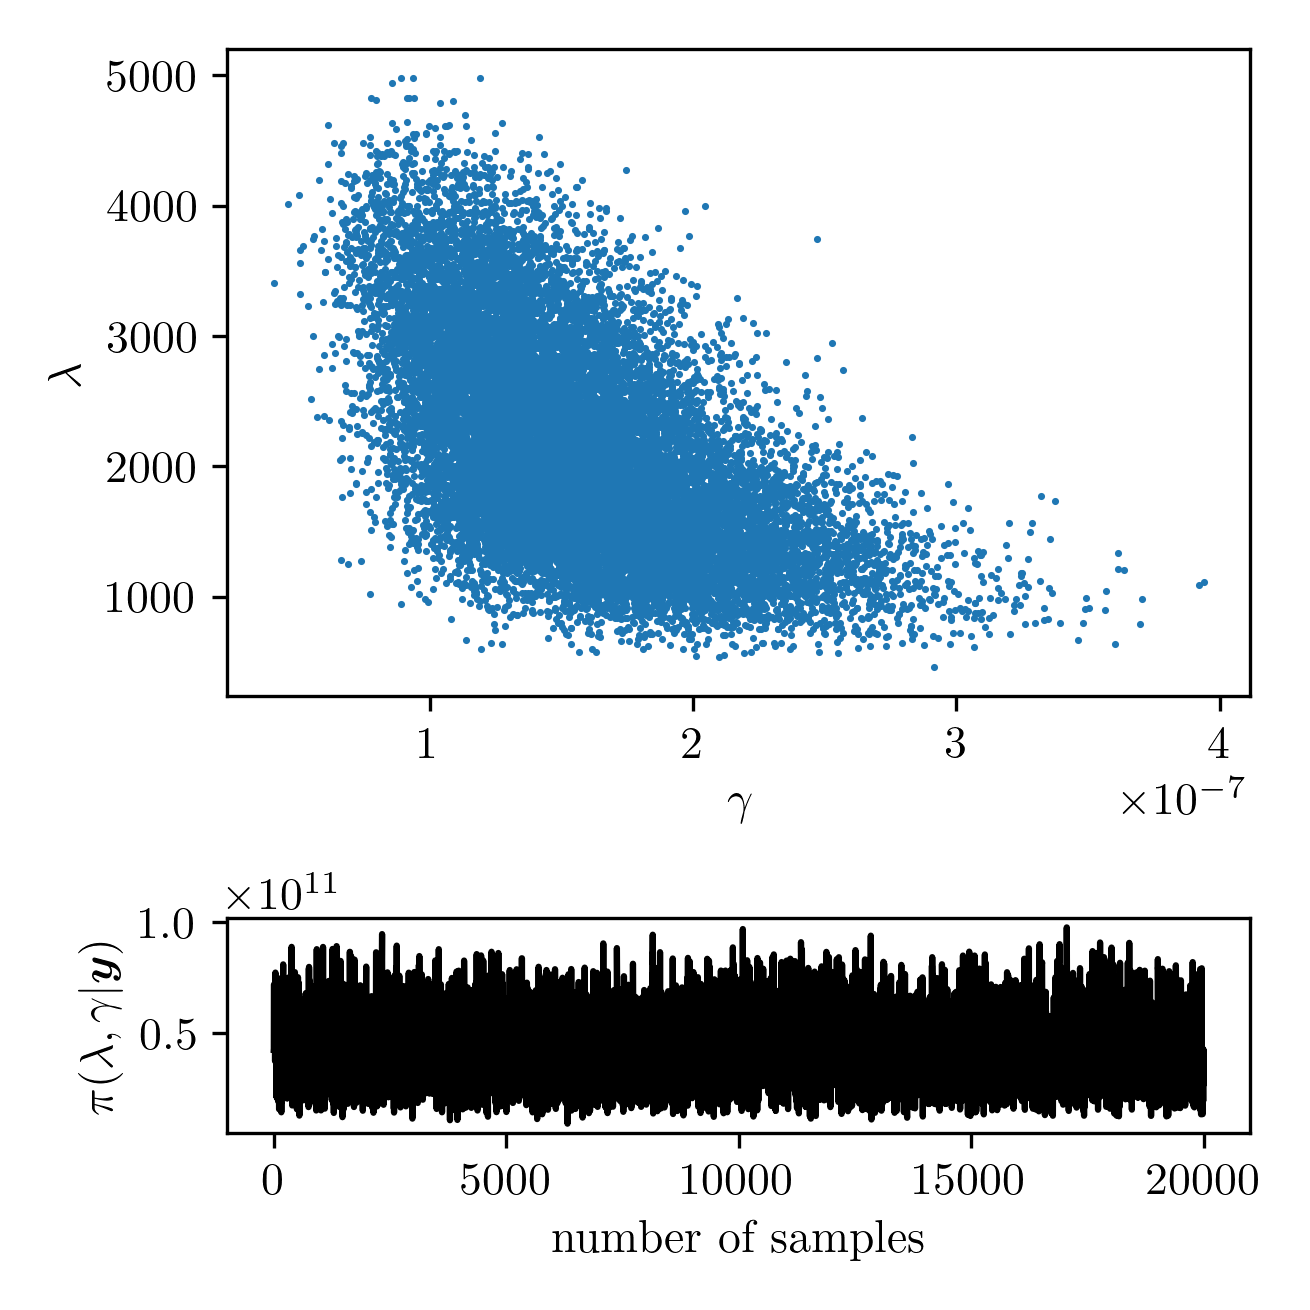
\includegraphics{ScatterplusHisto.png}
	\caption[]{}
	\label{fig:}
\end{figure}

\subsubsection{sampling from conditional posterior Posterior}
\begin{itemize}
	\item draw samples using RTO, when variance is hard to calculate
	\item or calc mean and variance using see other section
\end{itemize}
\begin{figure}[ht!]
	\centering
	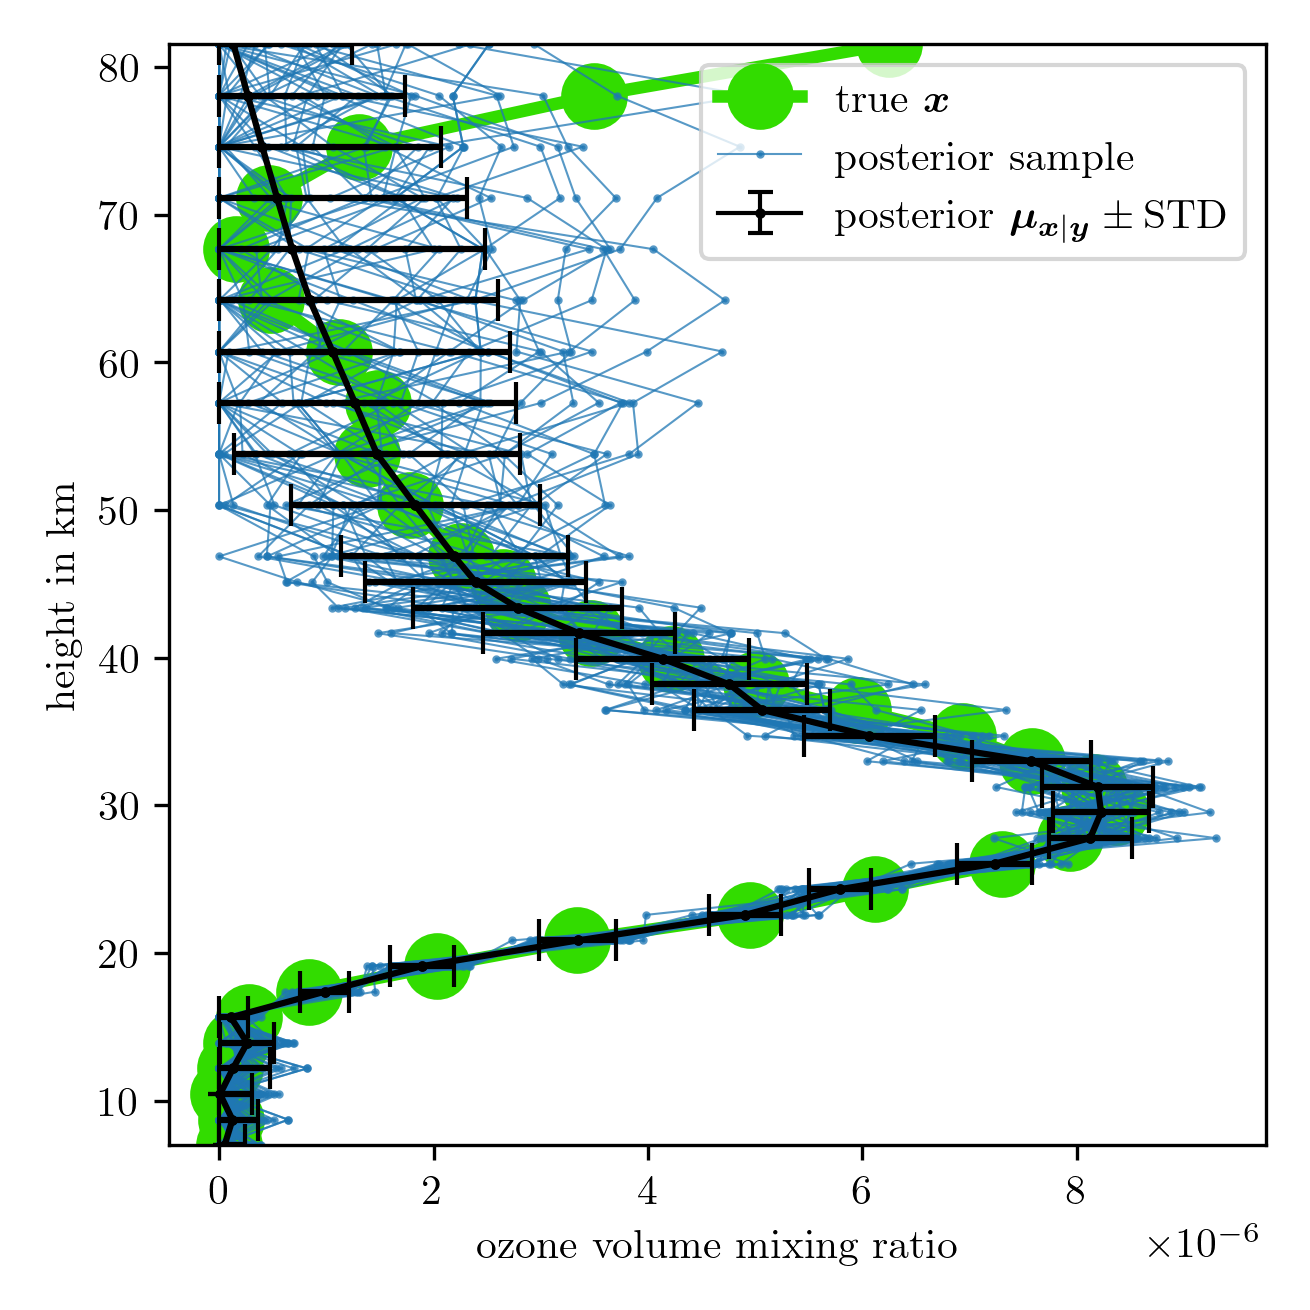
\includegraphics{FirstTestRes.png}
	\caption[]{}
	\label{fig:}
\end{figure}


\subsection{Asses Affine Map}
\begin{figure}[ht!]
	\centering
	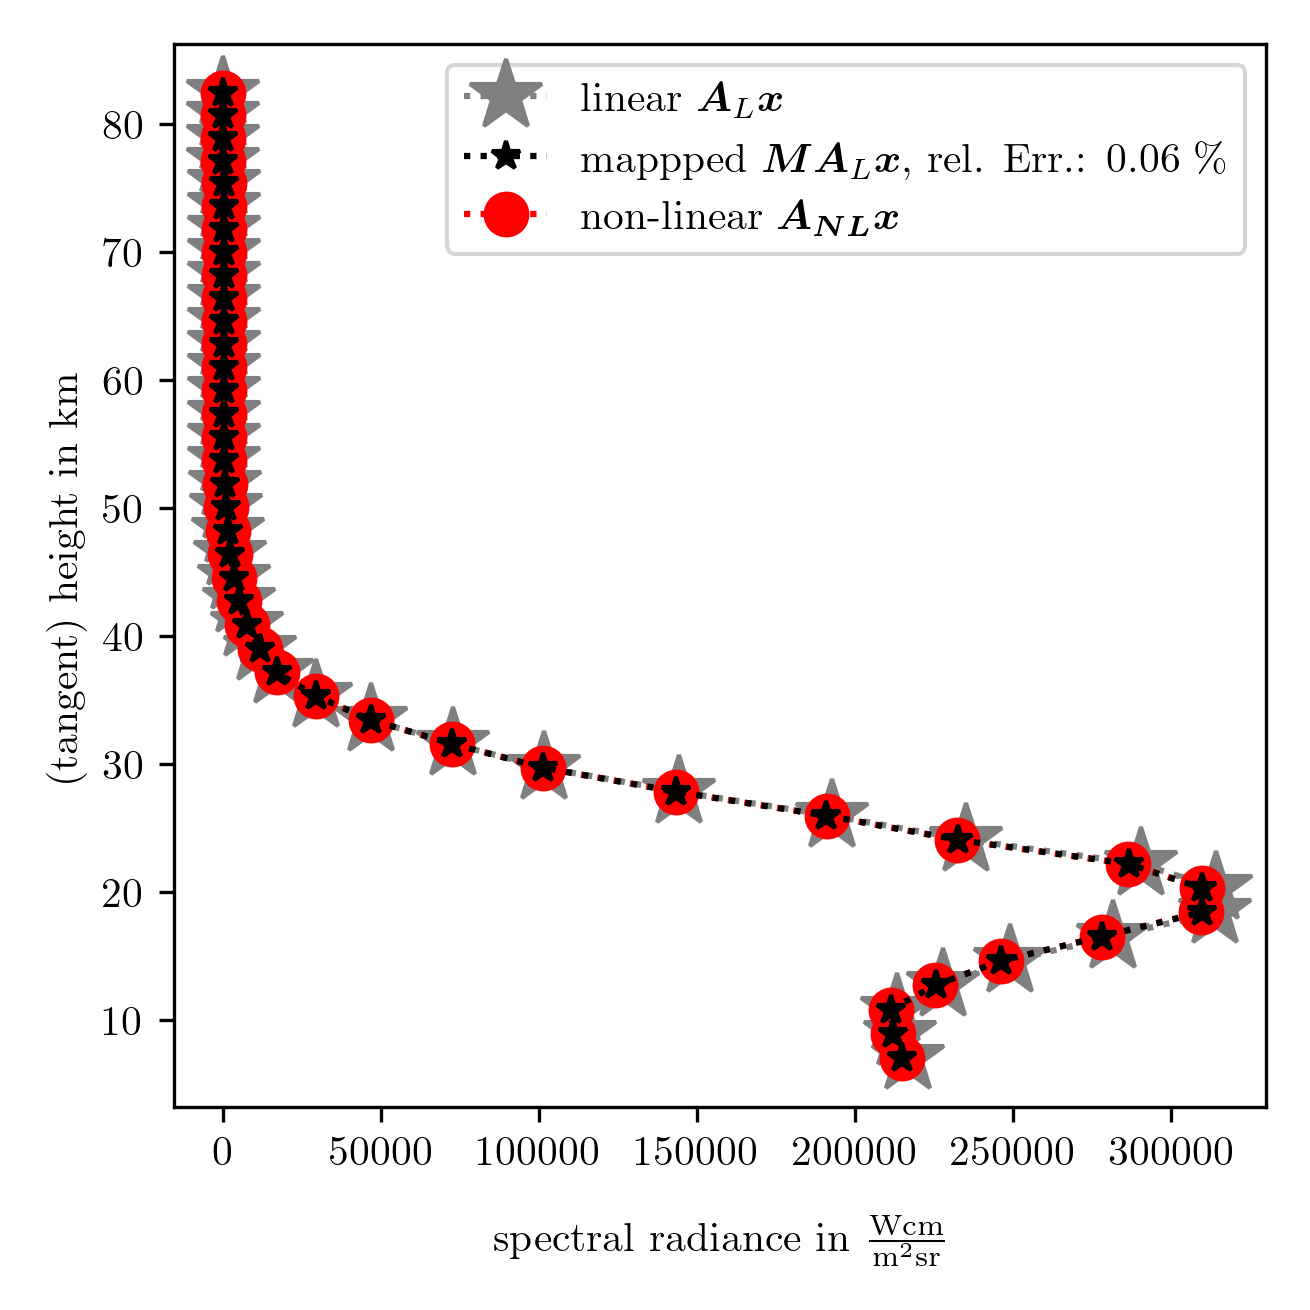
\includegraphics{SampMapAssesment.png}
	\caption[]{}
	\label{fig:}
\end{figure}


\section{Updated Forward map}

\begin{itemize}
	\item updated forward map
		\item do mtc again and then condition on pressure and temperature, samples
\end{itemize}


\subsection{Ozone Retrieval}
\begin{figure}[ht!]
	\centering
	\includegraphics{secRecRes.png}
	\caption[]{}
	\label{fig:}
\end{figure}

\subsubsection{MTC --  sampling vs TT}
\begin{figure}[ht!]
	\centering
	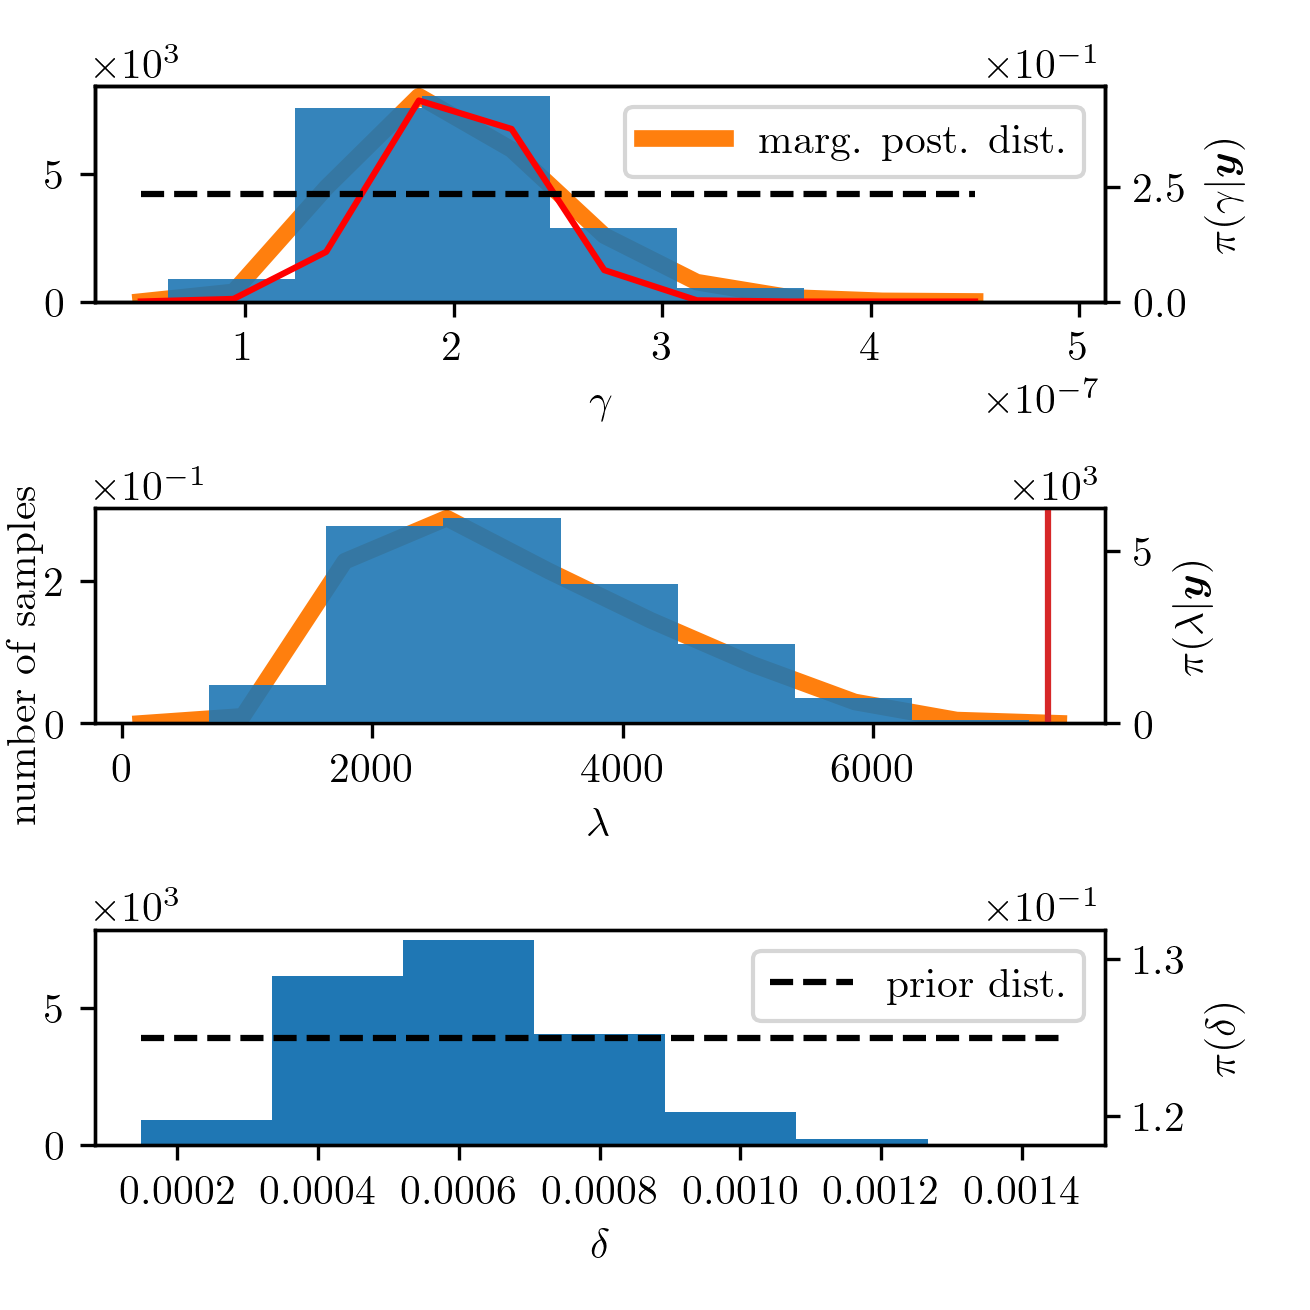
\includegraphics{secSIRTMargMargO3Res.png}
	\caption[]{}
	\label{fig:}
\end{figure}
\subsubsection{Regularized Solution}
\begin{itemize}
	\item similar to MTC model
	\item picture of L-Curve and samples 
	\item include in reg paraemter in histograms
\end{itemize}

\begin{figure}[ht!]
	\centering
	%\includegraphics{Reg.png}
	\caption[]{}
	\label{fig:}
\end{figure}
\subsection{Posterior Pressure and Temperature}
\begin{itemize}
	\item make table with set up for TT and sampling t-walk
	\item talk to colin about Error
\end{itemize}
\begin{figure}[thb!]
	\centering
	\begin{tikzpicture}
		
		\node[align=center] at (-1,4) (A)    {$\bm{M A}_L$};
		\node[roundnode2] at (-1,2.5) (u)    {$\bm{u}$};
		\node[rectnode] at (-1,1) (y)    {$\bm{y}$};
		
		\node[roundnode2] at (3,6.5) (t)     {$\bm{T}$};
		\node[roundnode2] at (-1,6.5) (p)     {$\bm{p}$};
		\node[roundnode2] at (1,5) (pt)     {$\bm{p}/\bm{T}$};
		\node[roundnode2] at (0,8) (b1)    {$b$};
		%\node[roundnode2] at (1,8) (b2)    {$b_2$};
		\node[roundnode2] at (-2,8) (h1)    {$h_0$};
		\node[roundnode2] at (-1,8) (p0)    {$p_0$};
		\node[roundnode2] at (2.25,8) (ht)    {$\bm{h_T}$};
		\node[roundnode2] at (3.25,8) (ct)    {$\bm{c_T}$};
		\node[roundnode2] at (4.25,8) (at)    {$\bm{a_T}$};
		
		%Lines
		\draw[->, very thick] (u.south) -- (y.north);
		\draw[->, mydotted, very thick] (A.south) -- (u.north);
		
		\draw[->, very thick] (p.south east) -- (pt.north west);
		\draw[->, very thick] (t.south west) -- (pt.north east);
		\draw[->,  mydotted, very thick] (pt.south west) -- (A.east);
		\draw[->, very thick] (h1.south) -- (p.north west);
		\draw[->, very thick] (p0.south) -- (p.north);
		\draw[->, very thick] (b1.south) -- (p.north east); 
		%\draw[->, very thick] (b2.south) -- (p.east); 
		
		\draw[->, very thick] (ht.south) -- (t.north west);
		\draw[->, very thick] (ct.south) -- (t.north);
		\draw[->, very thick] (at.south) -- (t.north east);
		
		%\node[align=center] at (0.25,4) (f3) {$\approx \bm{M A}_L$};
	\end{tikzpicture} 
\caption[]{}
\end{figure}

\begin{figure}[ht!]
	\centering
	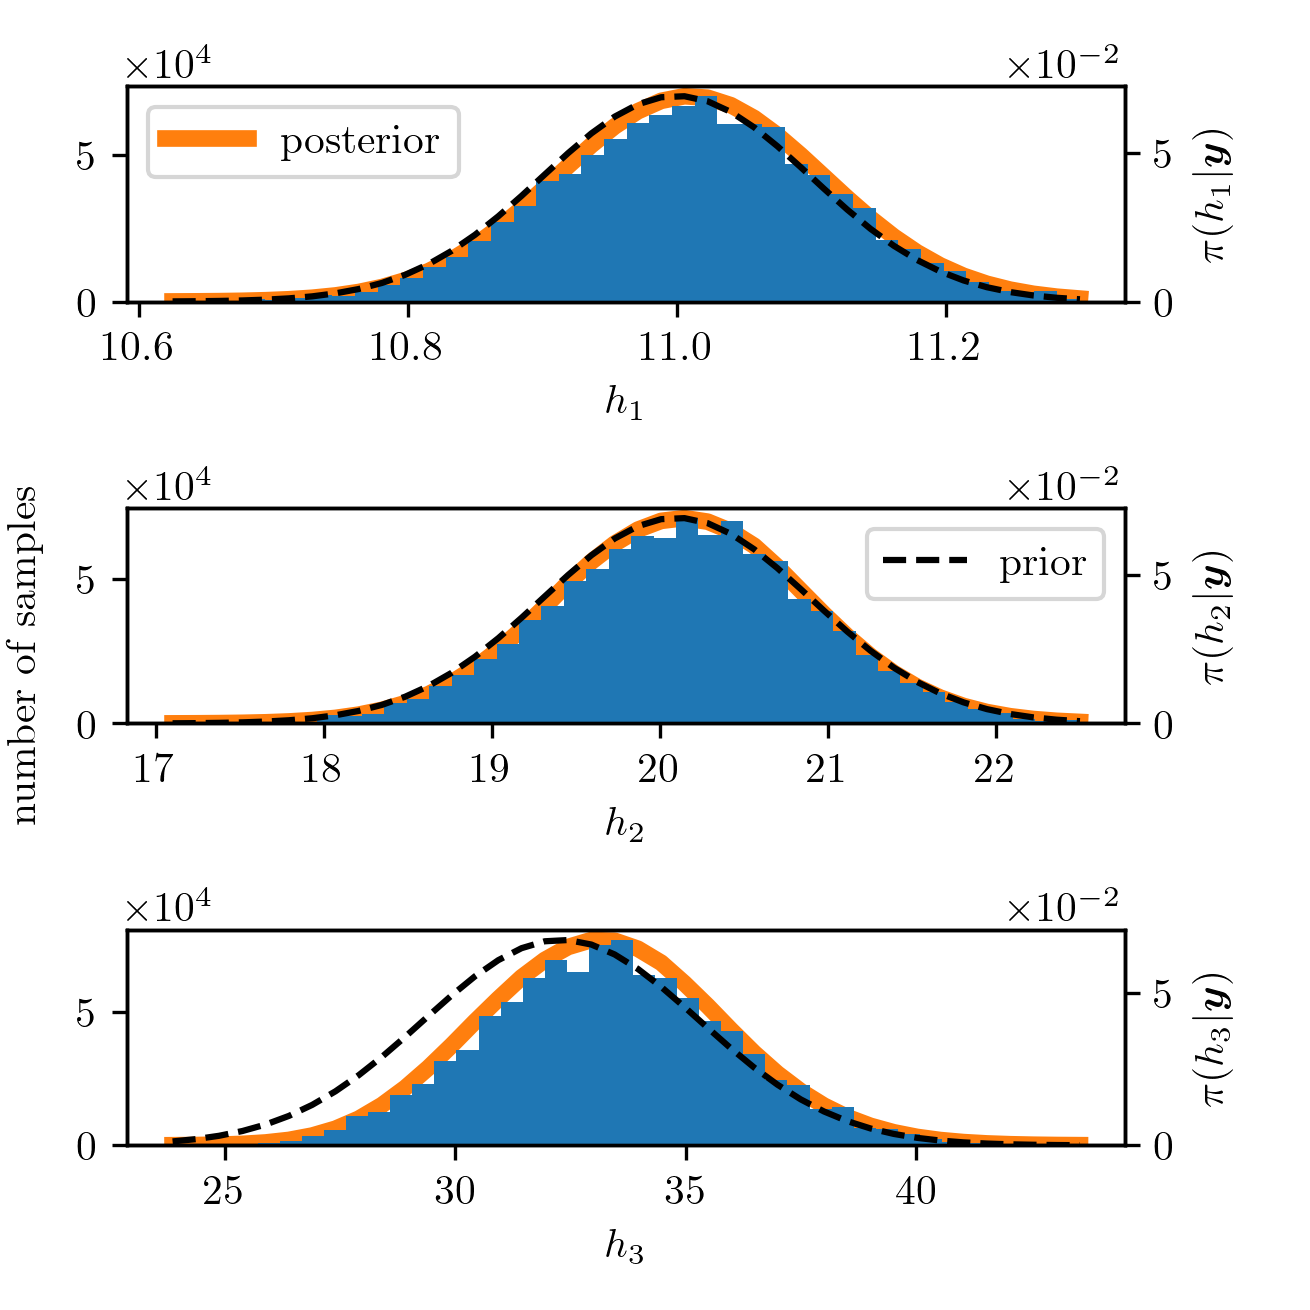
\includegraphics{PHdPTPost0.png}
	\caption[]{}
	\label{fig:}
\end{figure}
\begin{figure}[ht!]
	\centering
	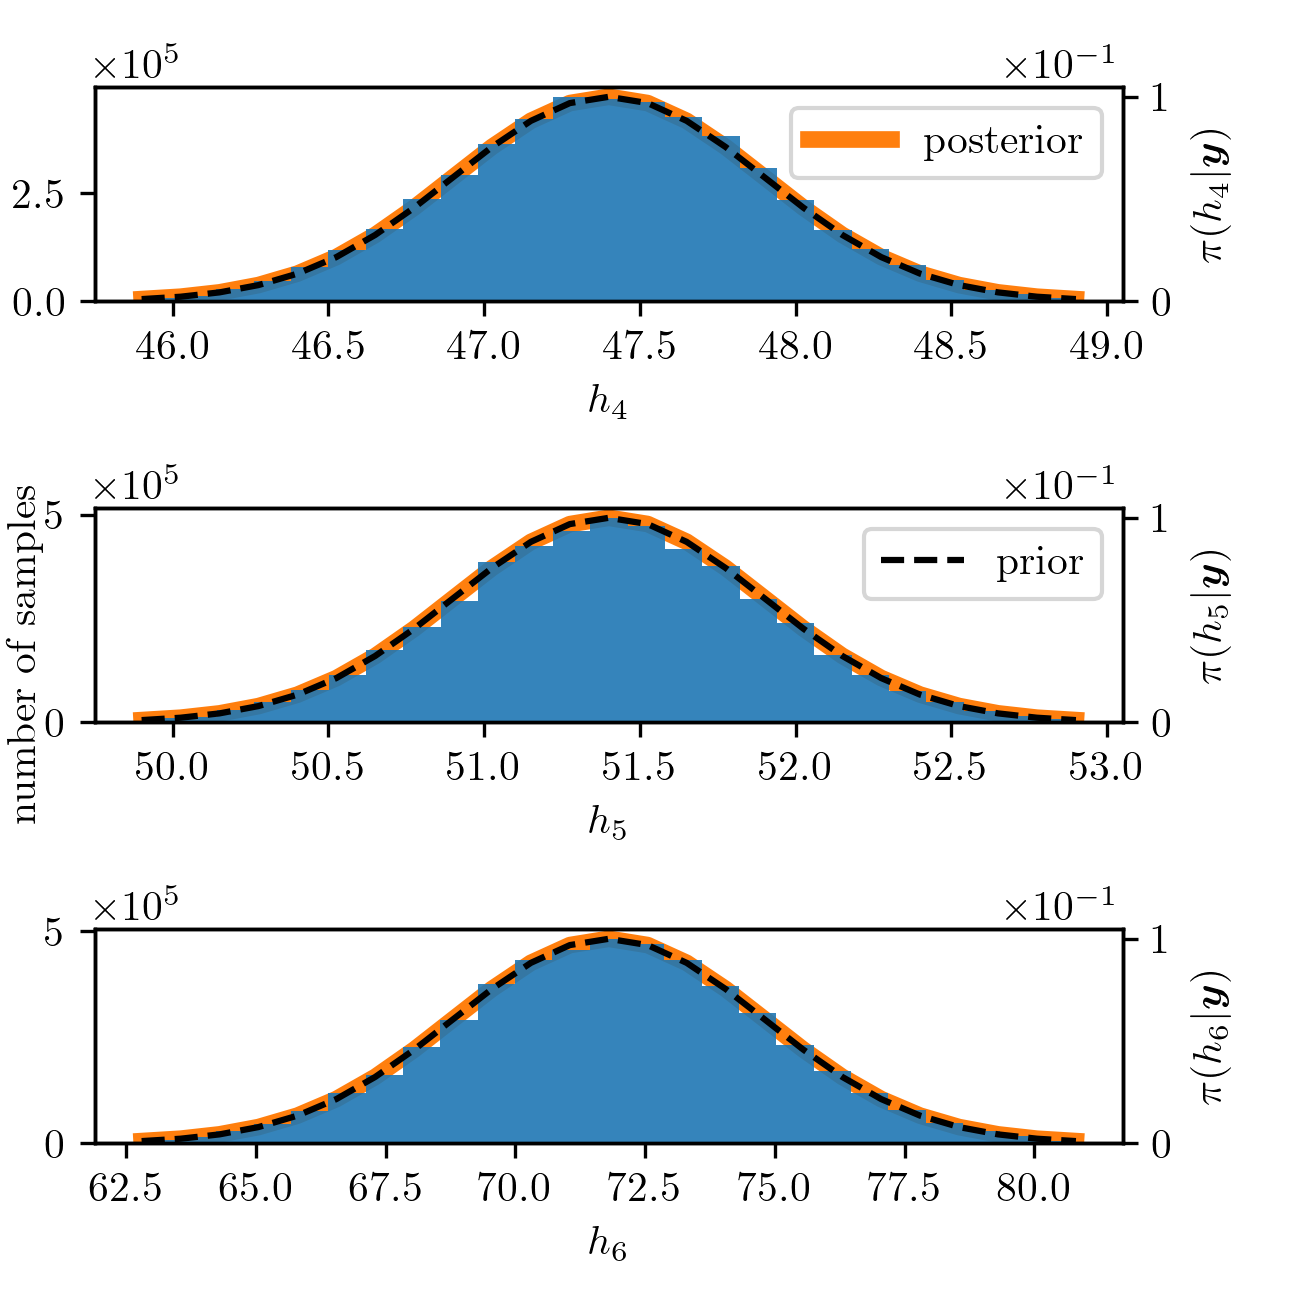
\includegraphics{PHdPTPost1.png}
	\caption[]{}
	\label{fig:}
\end{figure}
\begin{figure}[ht!]
	\centering
	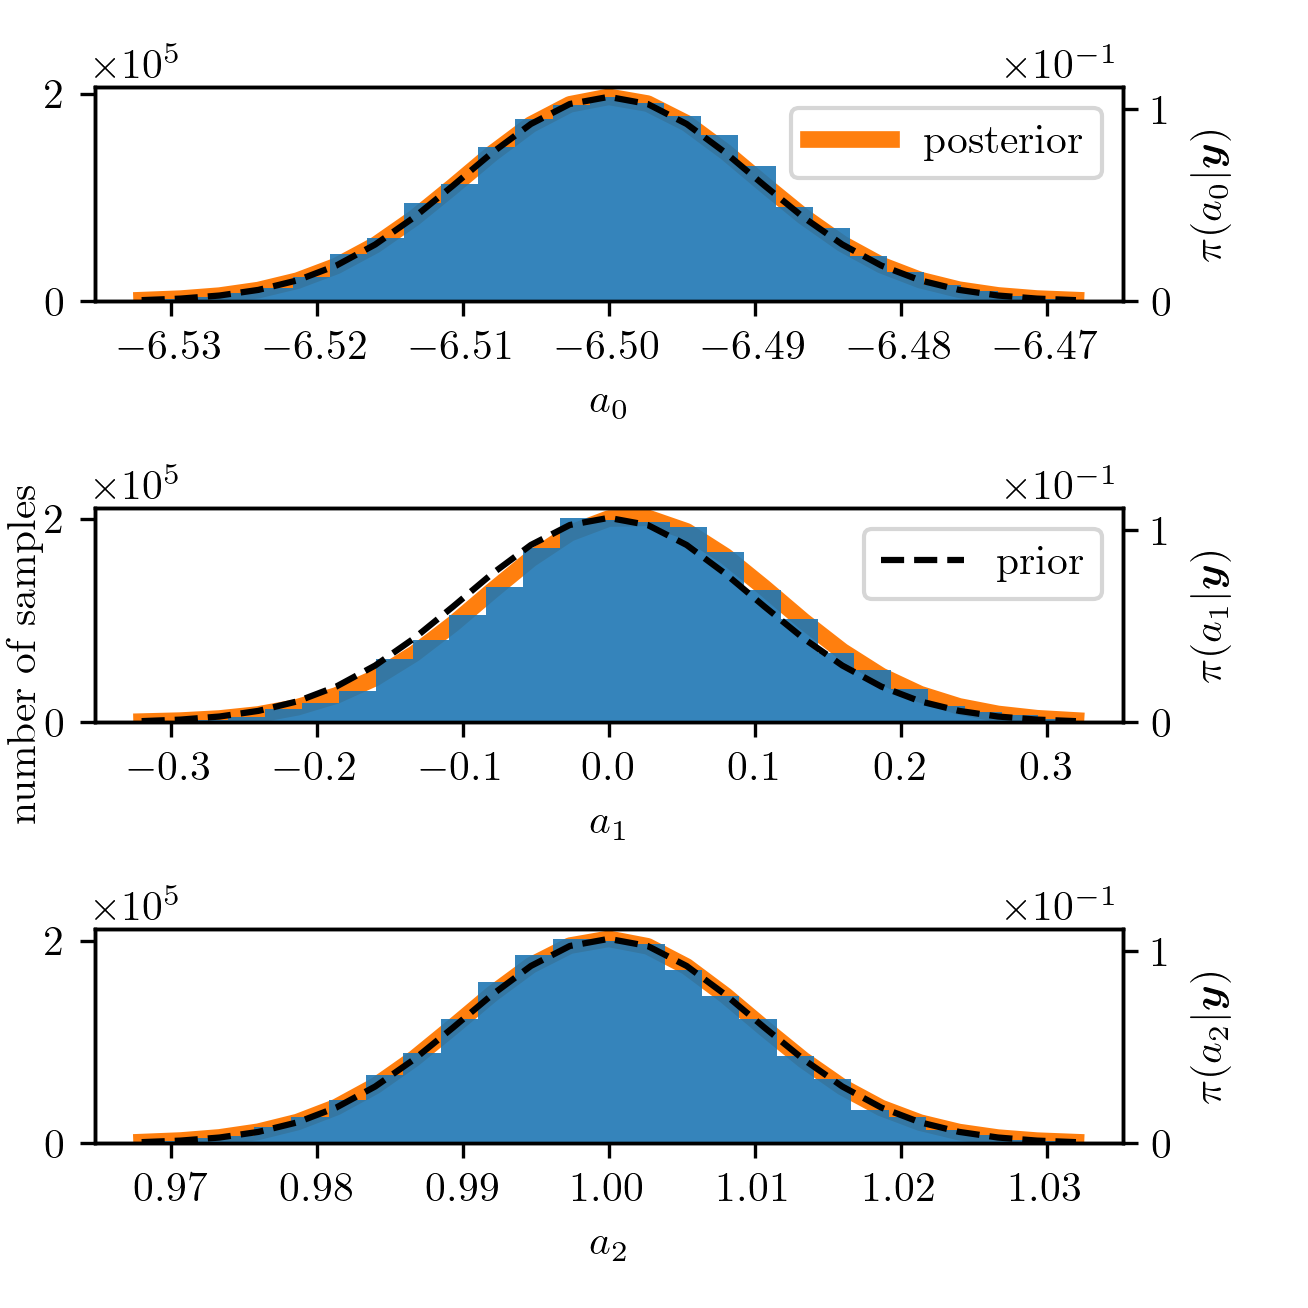
\includegraphics{PHdPTPost2.png}
	\caption[]{}
	\label{fig:}
\end{figure}
\begin{figure}[ht!]
	\centering
	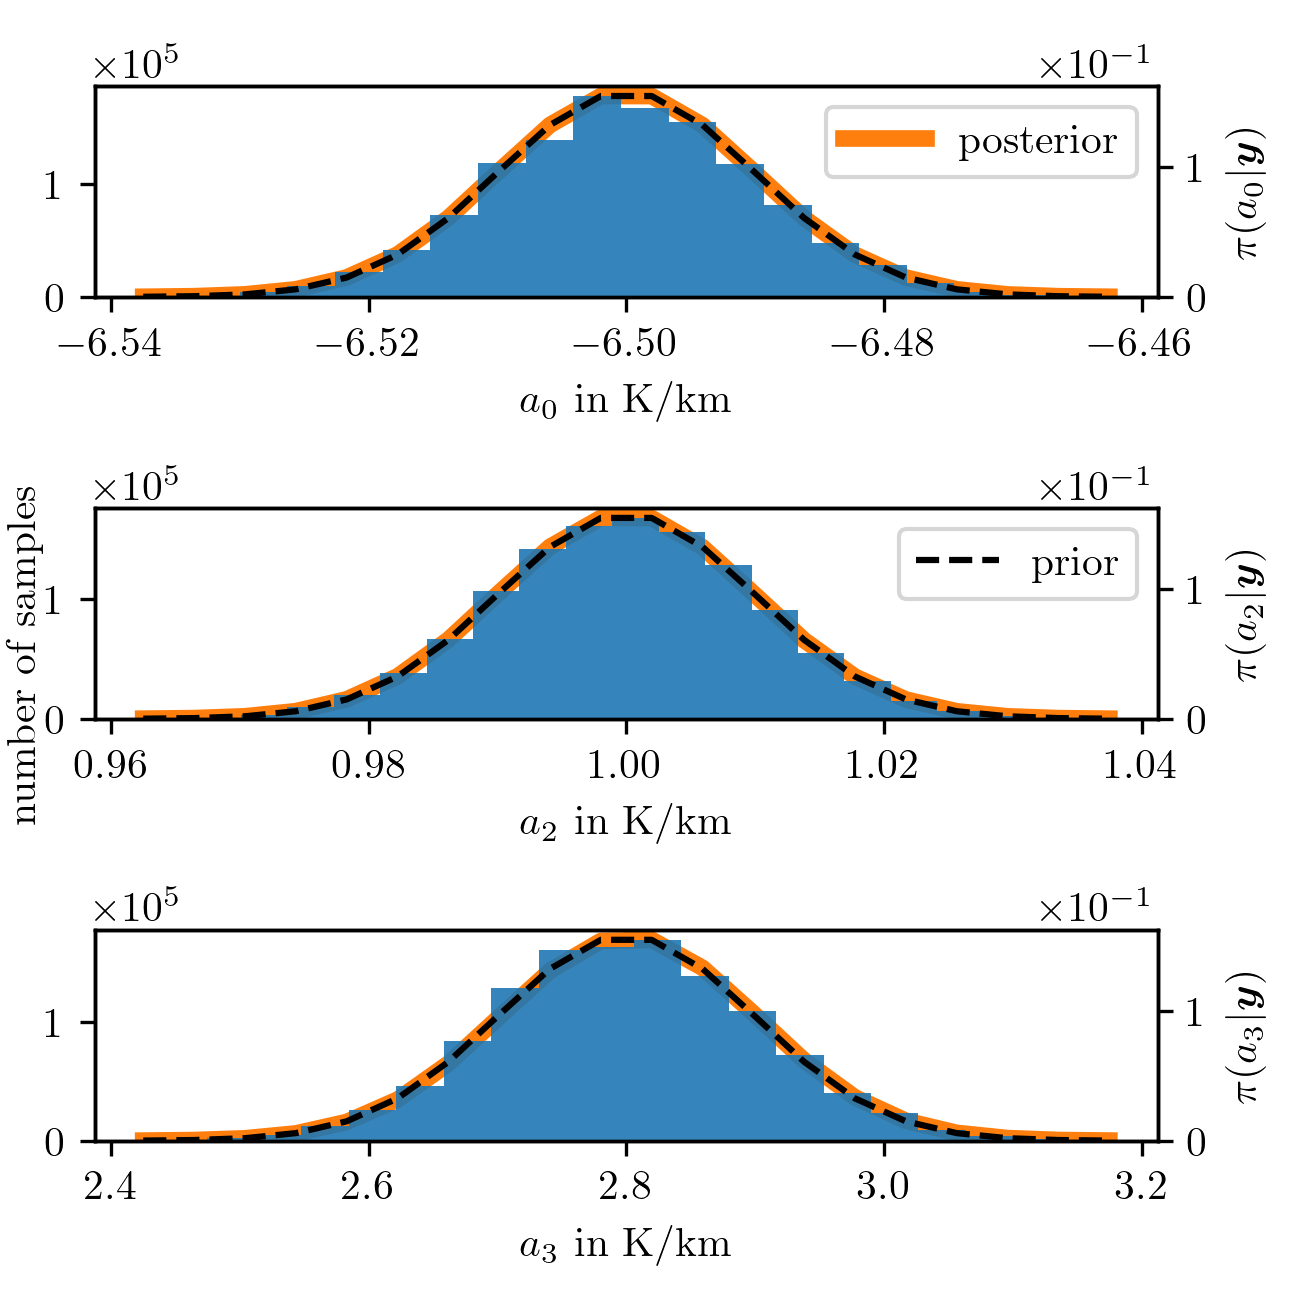
\includegraphics{PHdPTPost3.png}
	\caption[]{}
	\label{fig:}
\end{figure}
\begin{figure}[ht!]
	\centering
	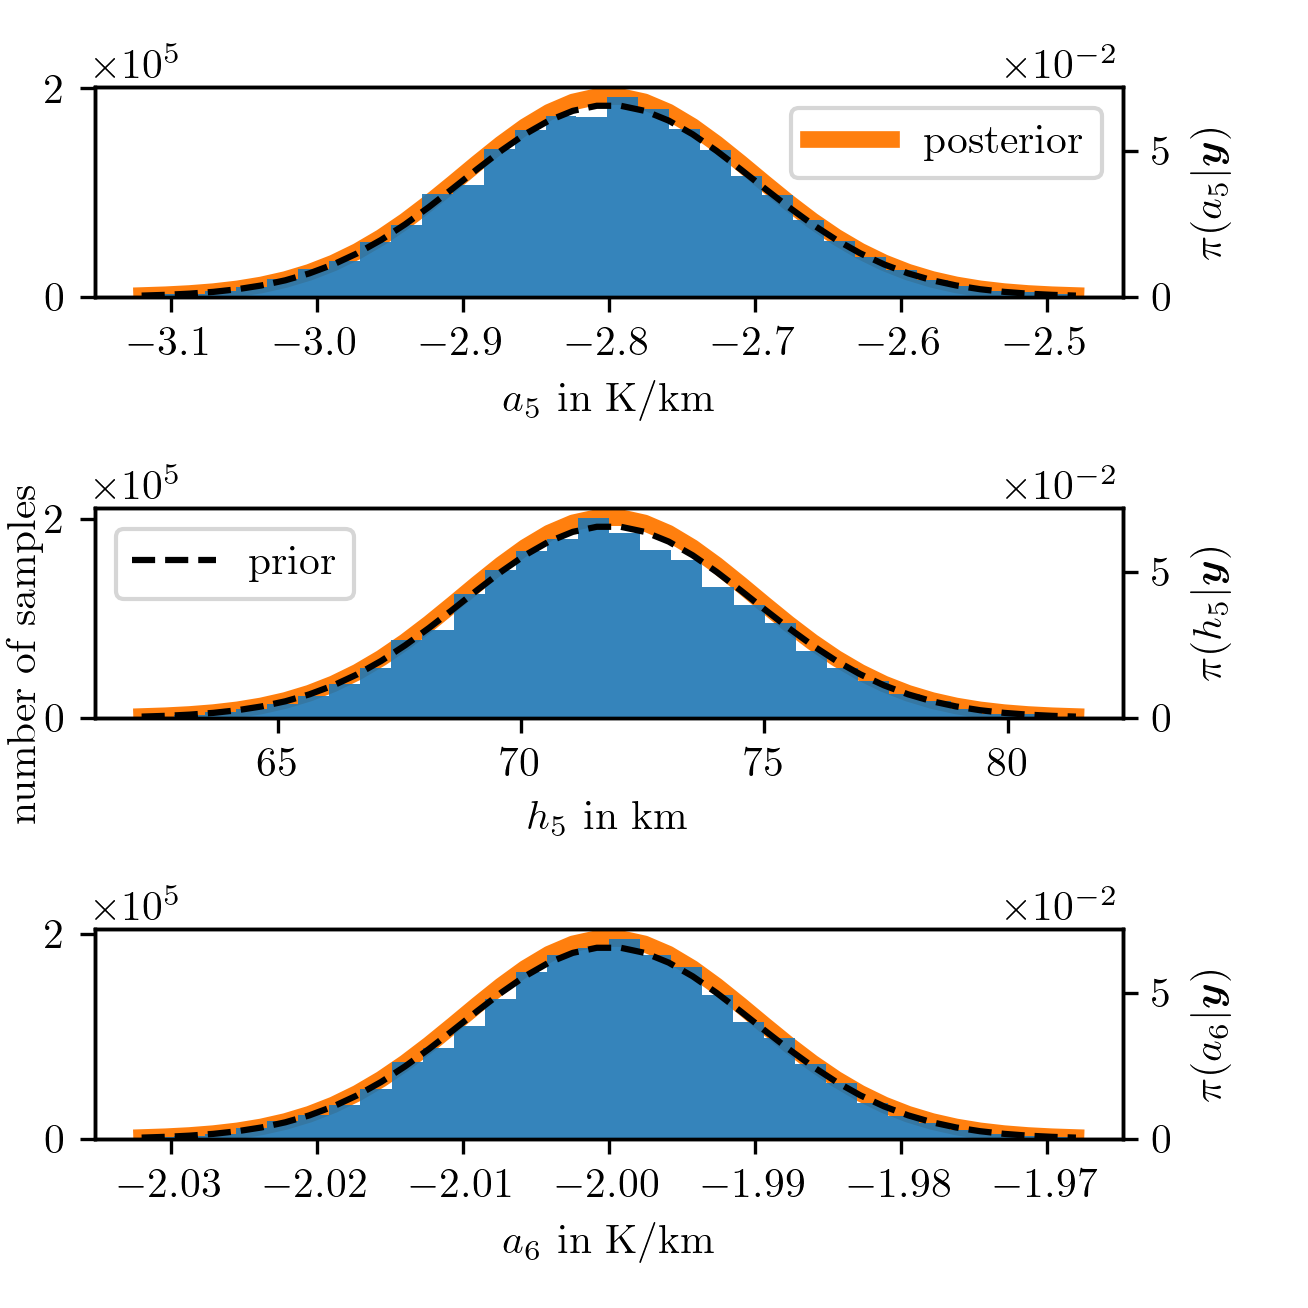
\includegraphics{PHdPTPost4.png}
	\caption[]{}
	\label{fig:}
\end{figure}

\begin{figure}[ht!]
	\centering
	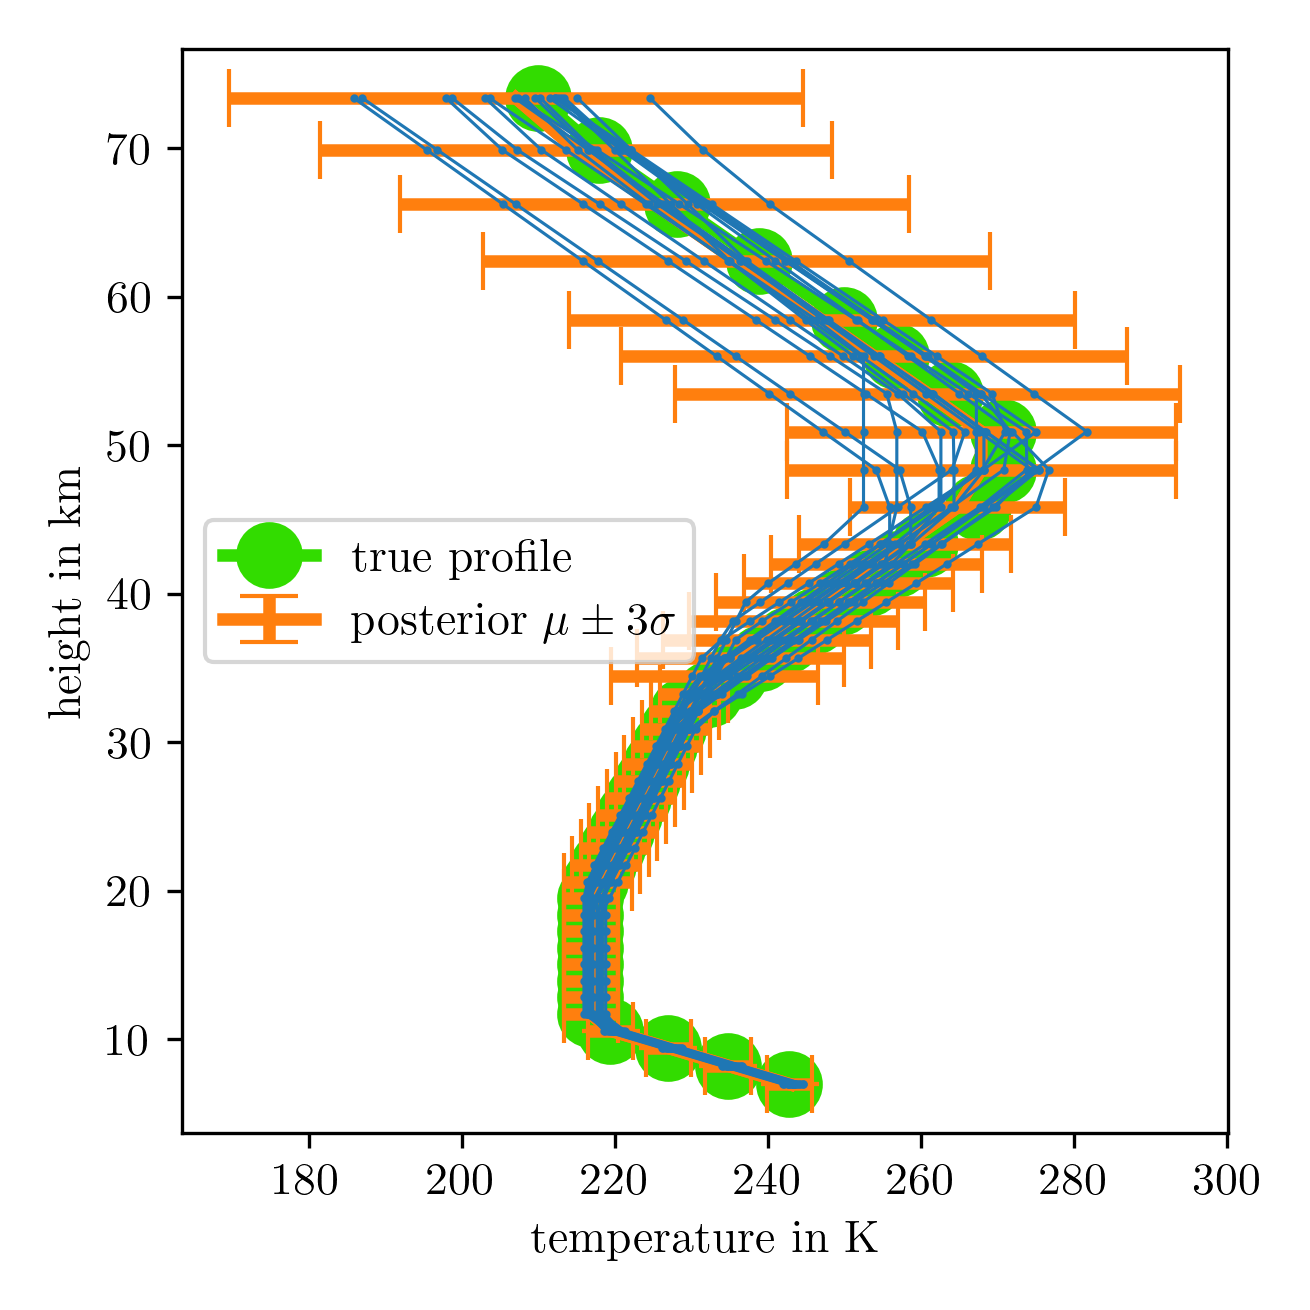
\includegraphics{TempPostMeanSigm.png}
	\caption[]{}
	\label{fig:}
\end{figure}

\begin{figure}[ht!]
	\centering
	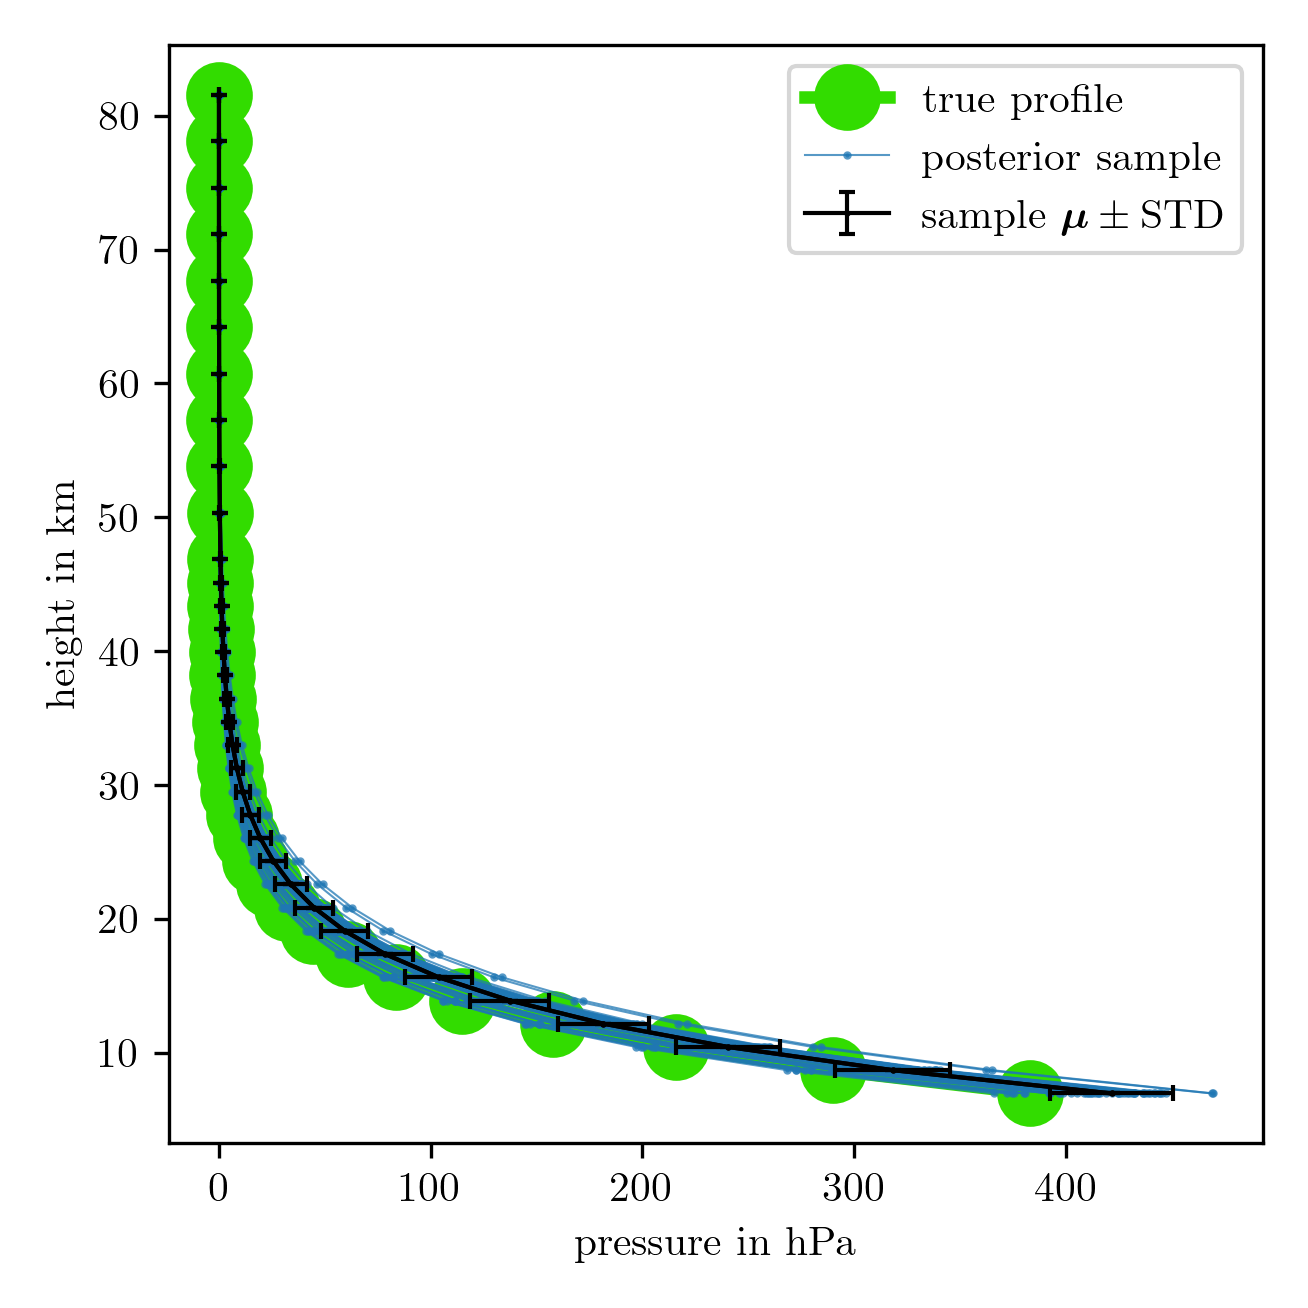
\includegraphics{PressPostMeanSigm.png}
	\caption[]{}
	\label{fig:}
\end{figure}



